\section{baba.vision}

\begin{frame}{Translating the research frontier}
    \begin{tikzpicture}
        \node[] at (-5.25, 3.5) {};
        \node[] at (5.25, -3.5) {};

        \only<1>{
            \node[text width=10.5cm] at (0, 0) {
                There are several challenges to translating AI models from the research frontier into real-world clinical applications.
                \begin{itemize}
                    \item \textbf{Lacking explainability.}
                    \item The models are not tailored for clinical use-cases.
                    \item The models are trained using data collected for research purposes.
                \end{itemize}
            };
        }

        \only<2>{
            \node[inner sep=0pt, draw=black] at (0, 0) {
                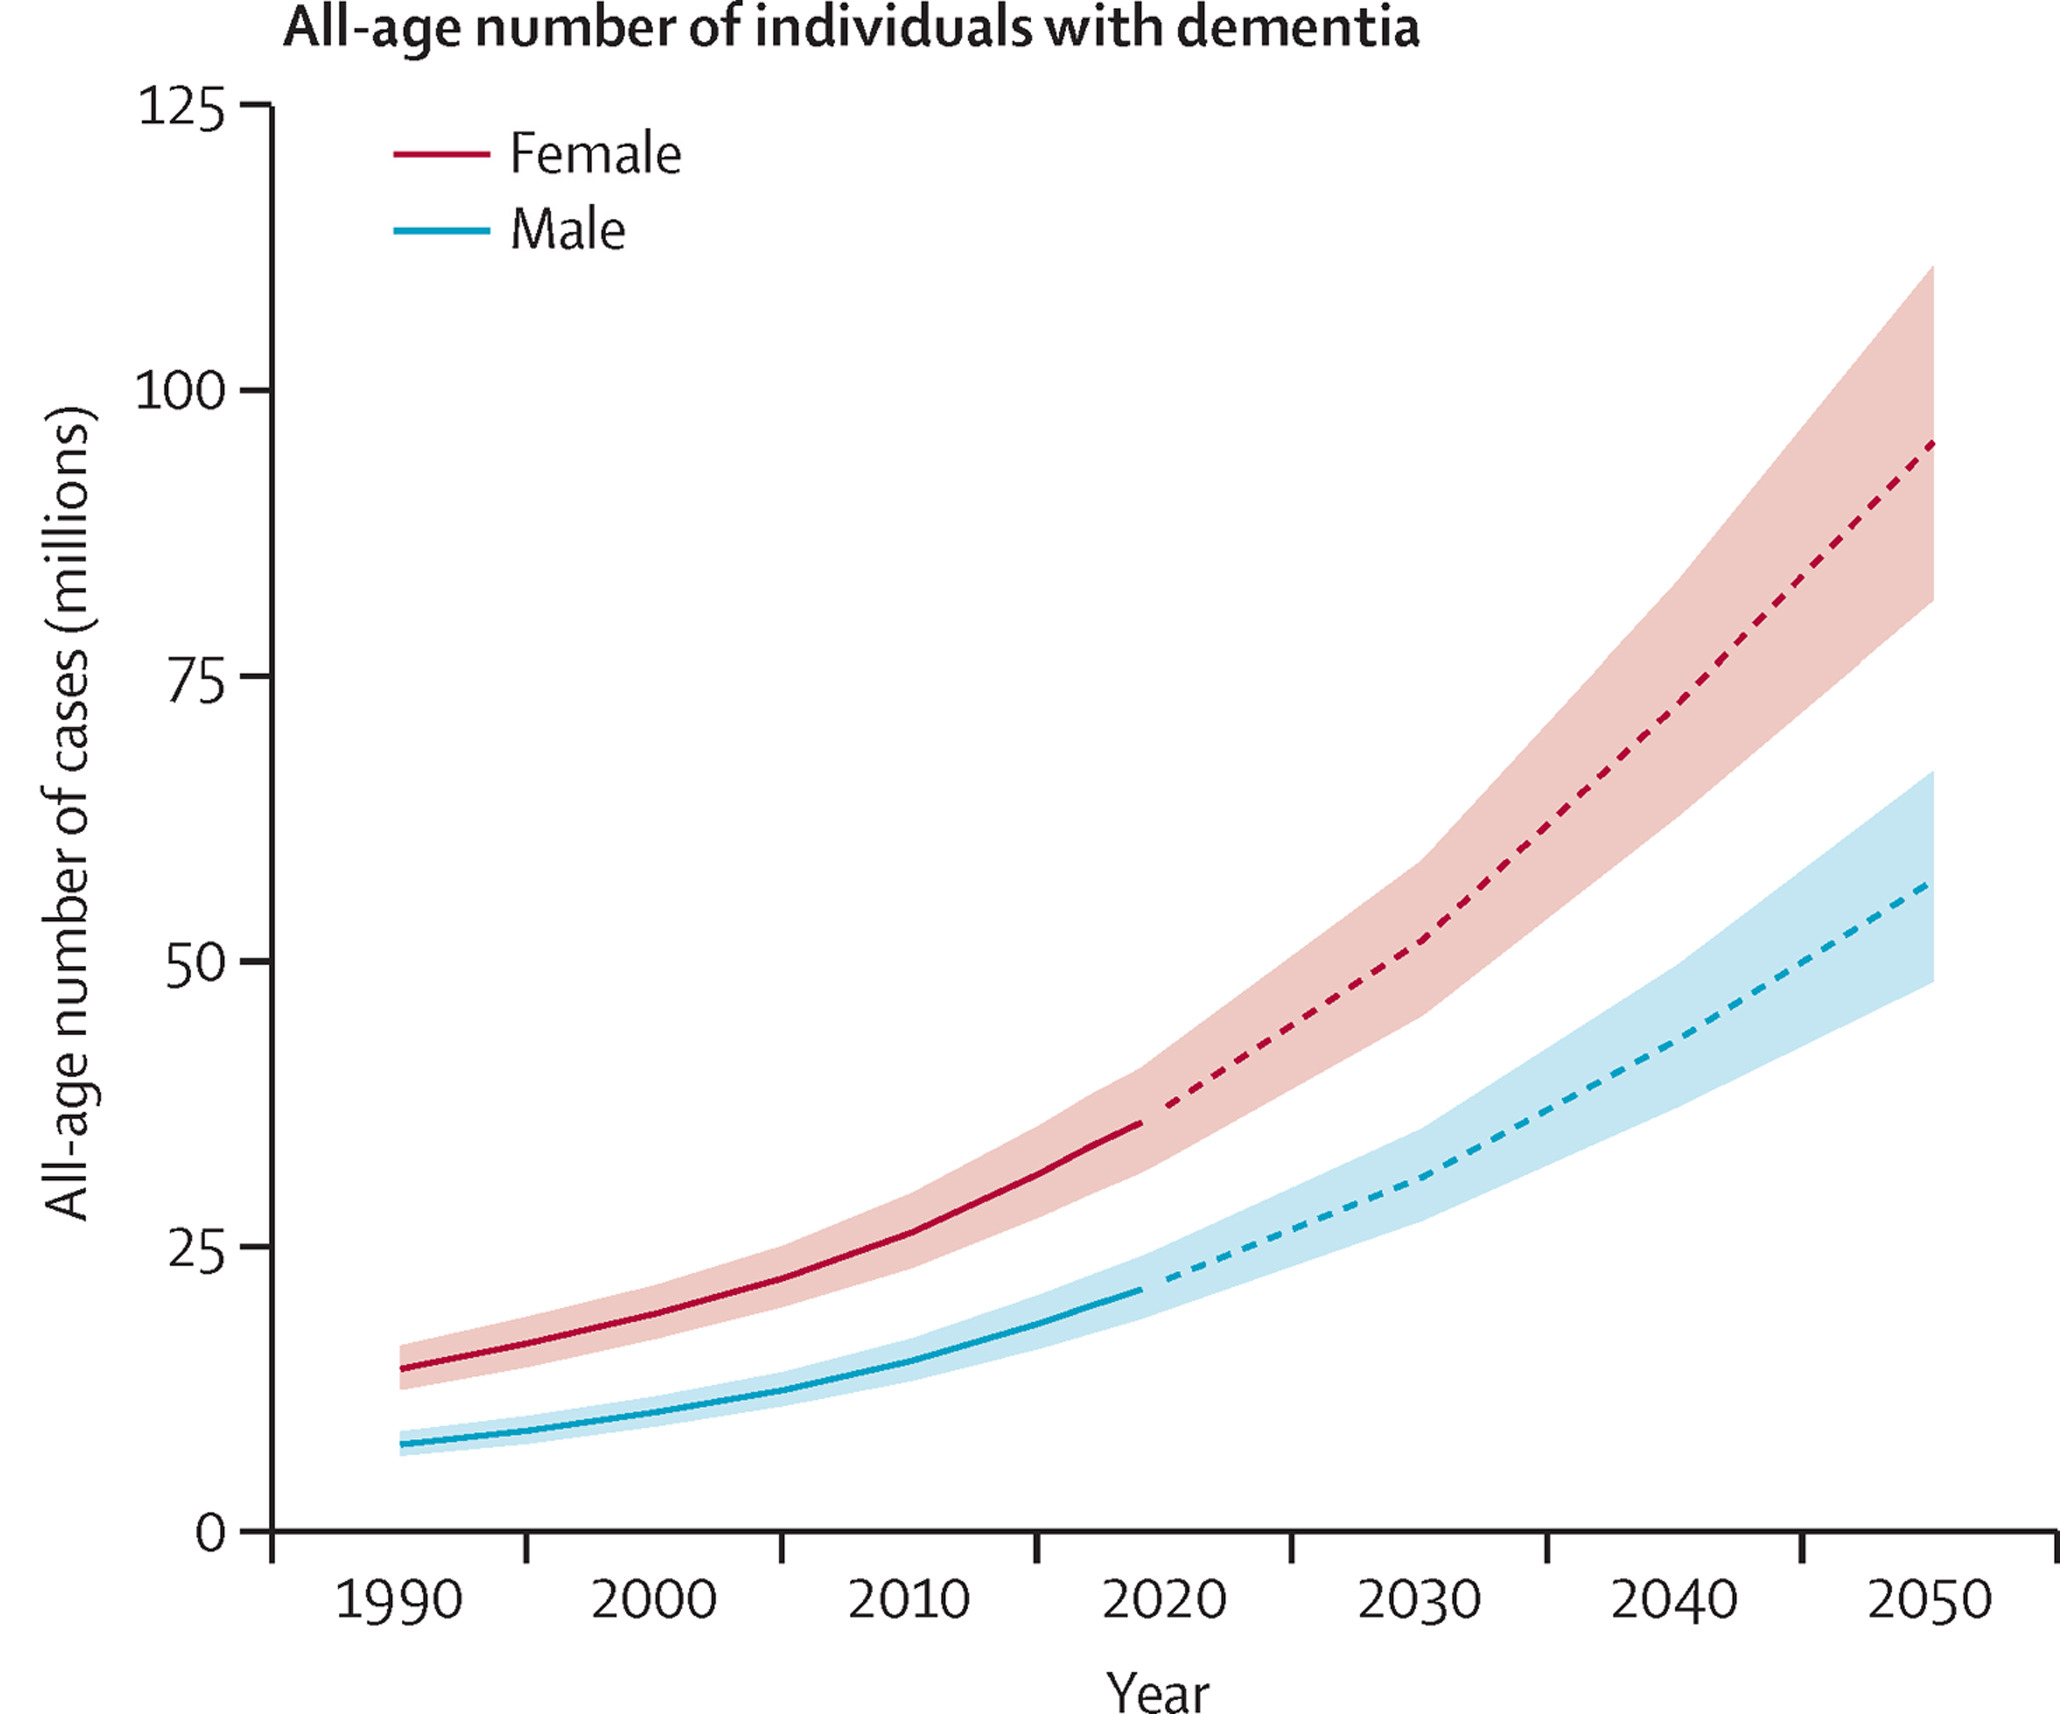
\includegraphics[width=6cm]{data/prevalence.jpg}
            };
            \node[anchor=south, font=\tiny, text width=10cm, align=flush center] at (0, -3.75) {
                Global Burden of Disease Dementia Forecasting Collaborators (2022). Estimation of the global prevalence of dementia in 2019 and forecasted prevalence in 2050: an analysis for the Global Burden of Disease Study 2019. \textit{The Lancet Public Health}.
            };
        }

        \only<3>{
            \node[inner sep=0pt, draw=black] at (0, 0) {
                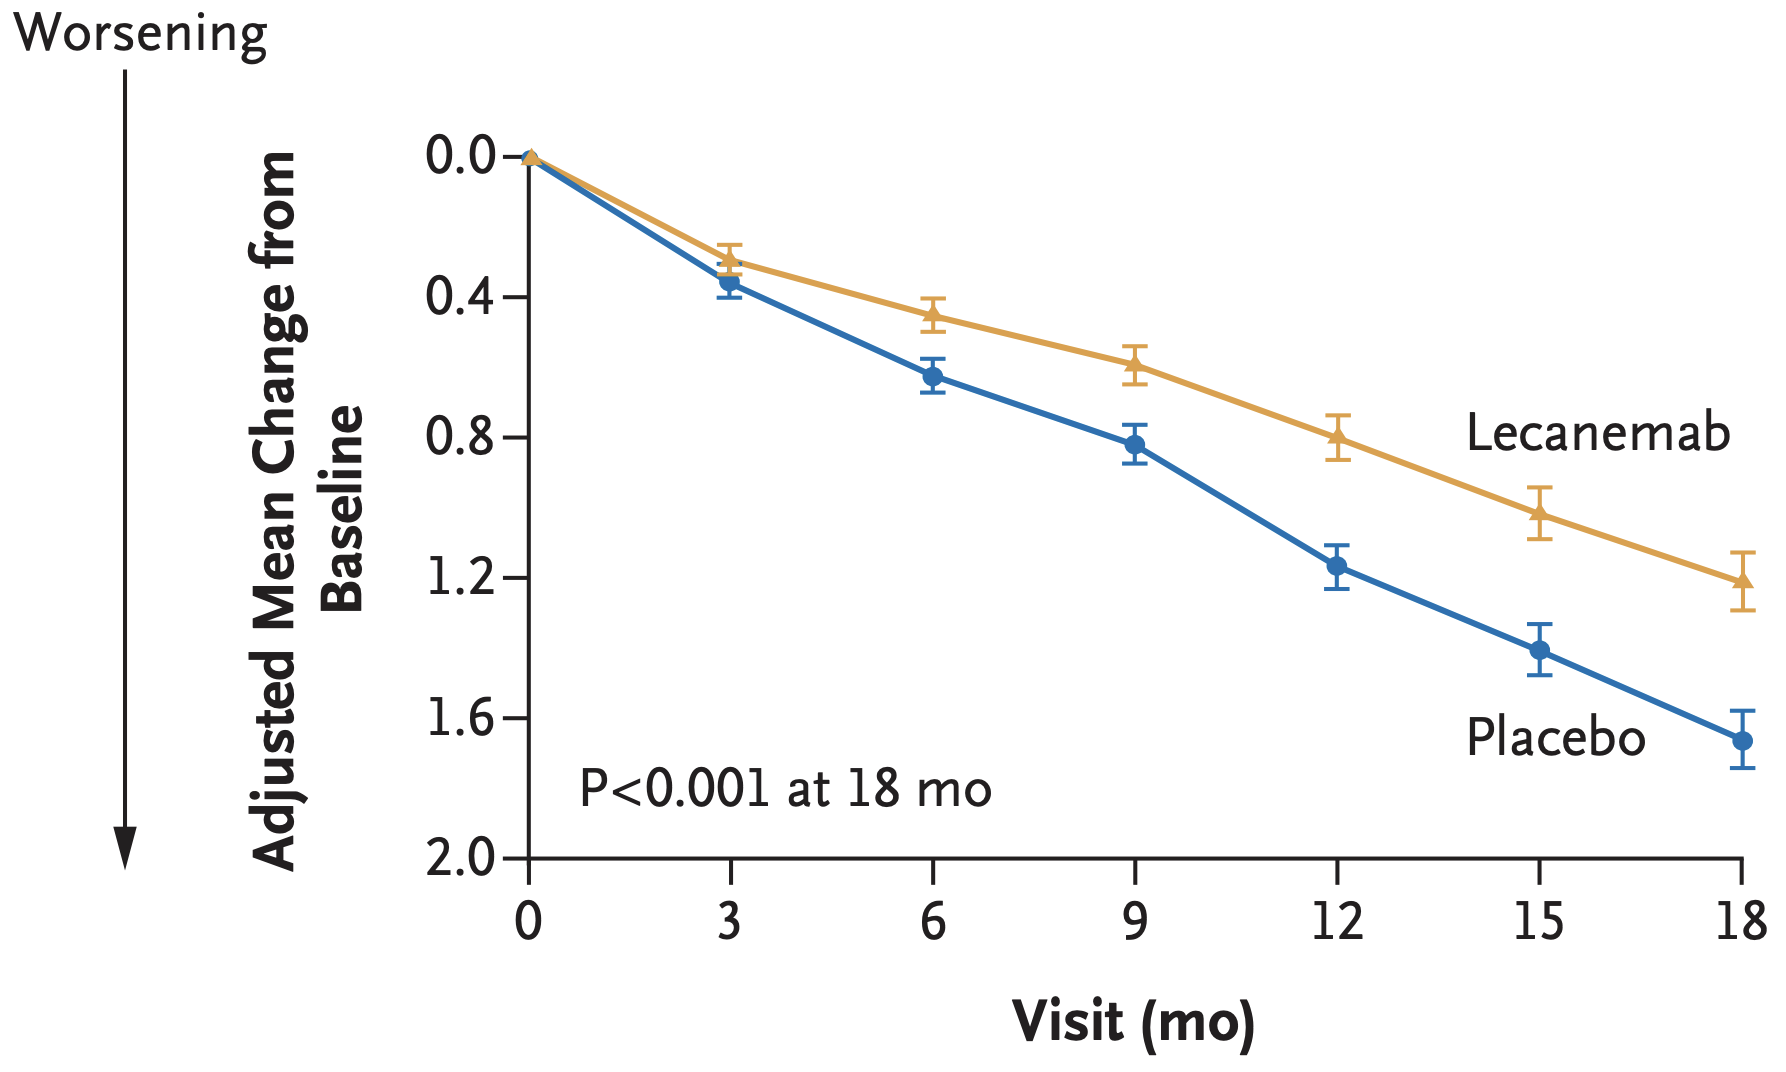
\includegraphics[width=8.5cm]{data/worsening.png}
            };
            \node[anchor=south, font=\tiny, text width=10cm, align=flush center] at (0, -3.75) {
                Van Dyck, C. H., Swanson, C. J., Aisen, P., Bateman, R. J., Chen, C., Gee, M., ... \& Iwatsubo, T. (2023). Lecanemab in early Alzheimer’s disease. \textit{New England Journal of Medicine}.
            };
        }
        \only<4>{
            \node[] at (0, 0) {
                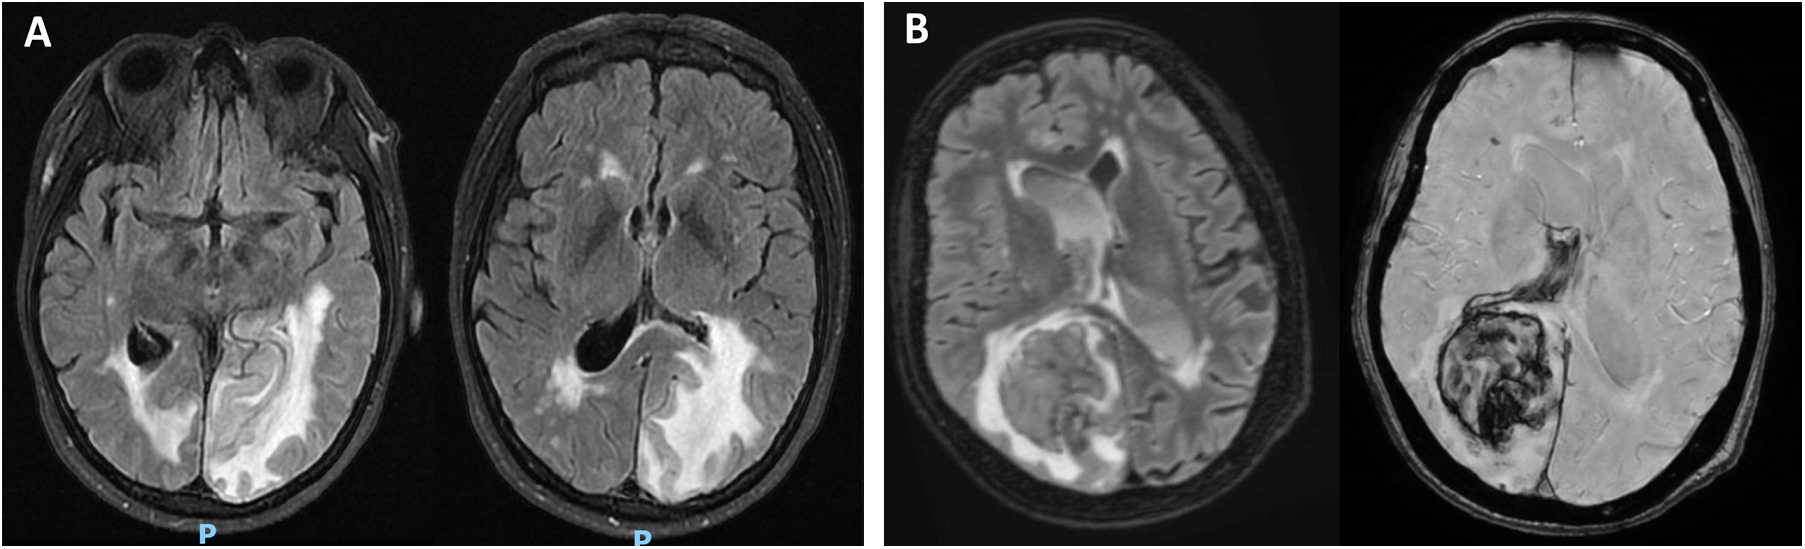
\includegraphics[width=10cm]{data/aria.jpg}
            };
            \node[anchor=south, font=\tiny, text width=10cm, align=flush center] at (0, -3.75) {
                Villain, N., Planche, V., \& Levy, R. (2022). High-clearance anti-amyloid immunotherapies in Alzheimer's disease. Part 1: Meta-analysis and review of efficacy and safety data, and medico-economical aspects. \textit{Revue neurologique}.
            };
        }
    \end{tikzpicture}
\end{frame}

\begin{frame}{baba.vision's treatment support suite}
    \begin{tikzpicture}
        \node[] at (-5.25, 3.5) {};
        \node[] at (5.25, -3.5) {};

        \only<1-3,5>{
            \node[inner sep=0pt, draw=black] at (0, 0) {
                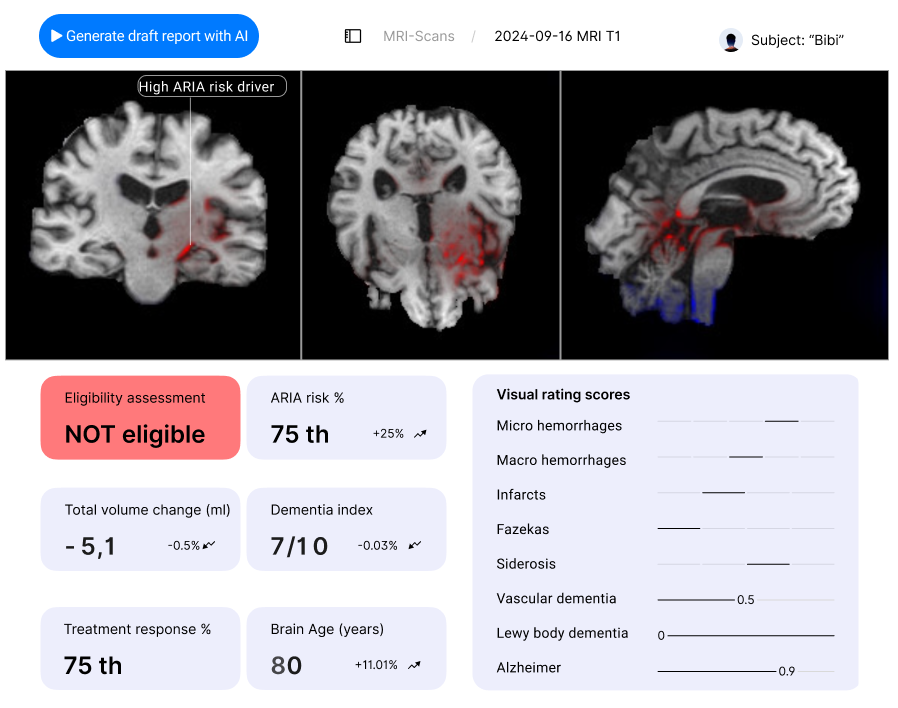
\includegraphics[width=8cm]{data/prototype.png}
            };
        }

        \only<2>{
            \node[minimum width=1.85cm, minimum height=0.8cm, draw=red, thick] at (-0.915, -2.62) {};
            \node[minimum width=1.85cm, minimum height=0.8cm, draw=red, thick] at (-0.915, -1.56) {};
        }

        \only<3>{
            \node[minimum width=3.3cm, minimum height=1.5cm, draw=red, thick] at (1.92, -1.25) {};
        }
        \only<5>{
            \node[minimum width=1.85cm, minimum height=0.8cm, draw=red, thick] at (-2.75, -2.62) {};
            \node[minimum width=1.85cm, minimum height=0.8cm, draw=red, thick] at (-0.915, -0.57) {};
        }
        \only<4>{
            \node[anchor=west, fill=babalightblue, text=white, align=center, font=\small, rounded corners=2pt, inner sep=5pt] (inhouse) at (-5.25, -1.5) {
                baba.vision's\\in-house dataset\\(40,000+ MRIs)
            };
            \node[anchor=west, fill=babalightblue, text=white, align=center, font=\small, rounded corners=2pt, inner sep=5pt] (clinical) at (-5.25, 1.2) {
                Tailored clinical\\datasets
            };
            \node[fill=babalightblue, text=white, align=center, font=\small, rounded corners=2pt, inner sep=5pt] (rig) at (0, -1.5) {
                baba.vision's AI\\training rig
            };
            \node[anchor=east, fill=babalightblue, text=white, align=center, font=\small, rounded corners=2pt, inner sep=5pt] (models) at (5.25, -1.5) {
                Clinically useful\\explainable AI\\models
            };

            \draw[densely dotted] (-5.25, 0) -- (5.25, 0);
            \node[anchor=south west, font=\footnotesize, inner sep=2pt] at (-5.25, 0) {
                Partners and collaborators
            };
            \node[anchor=north west, font=\footnotesize, inner sep=2pt] at (-5.25, 0) {
                baba.vision
            };

            \draw[-stealth, line width=2pt, gray] (inhouse) -- (rig);
            \draw[-stealth, line width=2pt, gray] (rig) -- (models);
            \draw[-stealth, line width=2pt, gray, dotted] (clinical) -| (rig);

        }
    \end{tikzpicture}
\end{frame}